\pdfoutput=1
\providecommand{\DoNotLoadEpstopdf}{}
\documentclass[11pt,a4paper]{article}
\usepackage[T1]{fontenc}
\usepackage[utf8]{inputenc}
\usepackage{lmodern,amsmath,amssymb,amsthm,mathtools}
\usepackage[margin=1.08in]{geometry}
\usepackage{booktabs,array,enumitem,microtype,xcolor,needspace,upquote,multicol}
\usepackage{tikz}
\usetikzlibrary{arrows.meta,positioning,calc}
\usepackage[hypcap=false]{caption}
\usepackage[unicode,colorlinks=true,linkcolor=blue!45!black,citecolor=blue!45!black,urlcolor=blue!45!black]{hyperref}
\setlength{\emergencystretch}{2em}
\setlist{nosep}
\setcounter{tocdepth}{1}
\makeatletter
\renewcommand*\@pnumwidth{2em}
\@clubpenalty=10000
\renewcommand*\l@section[2]{\addvspace{.15em}\@dottedtocline{1}{0pt}{2.4em}{\bfseries #1}{\bfseries #2}}
\makeatother
\newtheorem{theorem}{Theorem}[section]
\newtheorem{lemma}[theorem]{Lemma}
\newtheorem{proposition}[theorem]{Proposition}
\newtheorem{corollary}[theorem]{Corollary}
\newtheorem{maintheorem}{Theorem}
\renewcommand{\themaintheorem}{\Alph{maintheorem}}
\theoremstyle{definition}
\newtheorem{definition}[theorem]{Definition}
\theoremstyle{remark}
\newtheorem{remark}[theorem]{Remark}
\numberwithin{equation}{section}
\DeclareMathOperator{\supp}{supp}
\DeclareMathOperator{\dist}{dist}
\DeclareMathOperator{\Var}{Var}
\DeclareMathOperator{\Cov}{Cov}
\newcommand{\Z}{\mathbb Z}
\newcommand{\N}{\mathbb N}
\newcommand{\R}{\mathbb R}
\newcommand{\eps}{\varepsilon}
\newcommand{\one}{\mathbf 1}
\newcommand{\Pp}{\mathbb P}
\newcommand{\E}{\mathbb E}
\newcommand{\cG}{\mathcal G}
\newcommand{\osc}{\operatorname{osc}}
\newcommand{\logit}{\operatorname{logit}}
\newcommand{\logistic}{\operatorname{logistic}}
\newcommand{\TV}{\operatorname{TV}}
\colorlet{rxaccent}{orange!80!black}
\setlist[enumerate]{label=\textup{(\roman*)},leftmargin=2em,itemsep=3pt,topsep=4pt}
\setlist[itemize]{leftmargin=1.7em,itemsep=2pt,topsep=4pt}
\allowdisplaybreaks[2]
\raggedbottom
\clubpenalty=10000
\widowpenalty=10000
\displaywidowpenalty=10000
\hyphenation{Lemma Lemmas Theorem Theorems Proposition Propositions Definition Definitions}
\hypersetup{pdftitle={Every phase mixture recurs: The planar Ising model with random boundary spins},pdfauthor={Seth Douglas and Nidhal Mghirbi},pdfsubject={Random boundary conditions, chaotic size dependence and metastates}}
\title{Every phase mixture recurs\\The planar Ising model with random boundary spins}
\author{Seth Douglas \and Nidhal Mghirbi}
\date{Version 2.0.0, November 2026}
\begin{document}
\maketitle
\begin{abstract}
Which thermodynamic states recur when an Ising system grows through every square and its exterior spins are independent fair signs? We prove that every convex mixture of the plus and minus phases recurs almost surely in the two-dimensional nearest-neighbour model. The boundary bonds have the bulk coupling strength. The result holds at every fixed inverse temperature above the critical one, that is, throughout the region of phase coexistence. It proves the two-dimensional full-sequence conjecture of van Enter, Neto\v cn\'y and Schaap. For each fixed interior window of mixture weights, its probability at size $n$ is at least a positive constant times $n^{-1/2}$. The proof combines the random-line representation of the dual high-temperature model, a central majority that labels the phase with exponentially small error, uniqueness at a uniform wall, and a count of pivotal boundary changes with arbitrarily small effects on the phase odds. We also prove almost-sure convergence along all sizes to the favoured pure phase for each nonzero boundary bias, and recover the equal two-atom empirical metastate at every temperature of the ordered phase. Thus every mixture recurs, while the sizes near mixed states have density zero.
\end{abstract}
\begin{center}\resizebox{\textwidth}{!}{Claude Opus 5.5, GPT-6.1 Sol, GPT-6.2 Sol and GPT-6.2 Astra assisted with this work; the authors take responsibility for every claim.}\end{center}
{\small\tableofcontents}
\section{The question and the results}\label{sec:intro}
A square Ising system is given a boundary at each size determined by the restrictions of one independent sign field on $\Z^2$. Which infinite-volume Gibbs states can one observe along subsequences of \emph{all} square sizes? A preference of order $\sqrt n$ usually selects one pure phase. The question concerns the exceptional sizes at which the two phases have nearly equal free energies. We prove that these sizes realize every mixture weight.

The distinction between recurrence and frequency is essential. The empirical distribution of the finite-volume measures gives mass one half to each pure phase, yet its cluster set contains their entire segment (Figure~\ref{fig:segment}). A sequence can visit every interior neighbourhood infinitely often and spend a vanishing fraction of its time there.

\begin{figure}[ht]
\centering
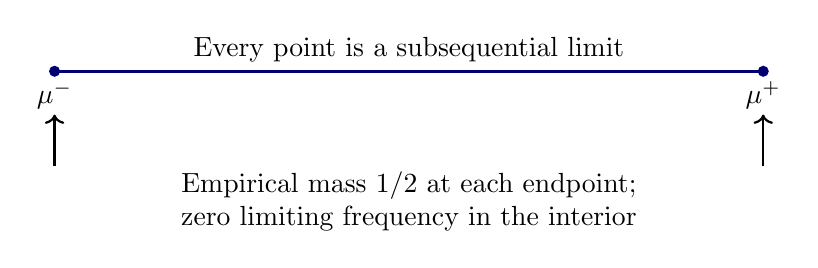
\begin{tikzpicture}[x=9cm,y=1cm]
\draw[very thick,blue!45!black] (0,0)--(1,0);
\fill[blue!45!black] (0,0) circle (2pt) (1,0) circle (2pt);
\node[below] at (0,0) {$\mu^-$};
\node[below] at (1,0) {$\mu^+$};
\node[above] at (.5,0) {Every point is a subsequential limit};
\draw[->,thick] (0,-1.2)--(0,-.55);
\draw[->,thick] (1,-1.2)--(1,-.55);
\node[below,align=center] at (.5,-1.15) {Empirical mass $1/2$ at each endpoint;\\zero limiting frequency in the interior};
\end{tikzpicture}
\caption{The cluster set and the empirical metastate describe different aspects of the same sequence. The drawing records the conclusions, rather than a finite-size probability density.}\label{fig:segment}
\end{figure}

Here is the range of the results. Let $K_c=\tfrac12\log(1+\sqrt2)=0.44068679\ldots$ be the critical inverse temperature of the planar nearest-neighbour model \cite{KW41,Onsager44}. Throughout the main results, $K$ is fixed and finite with $K>K_c$. This is the whole region in which the plus and minus phases coexist (for $K\le K_c$ the spontaneous magnetization vanishes \cite{Yang52,BGJS73} and the Gibbs state is unique \cite{LML72}).

Write $B_n=[-n,n]^2\cap\Z^2$, and let $\mu_n^\eta$ be the zero-field nearest-neighbour Gibbs measure with exterior spins $\eta$ and coupling $K$ on every bond meeting $B_n$. The signs $\eta_x$ are independent with $\Pp_p(\eta_x=+1)=p$. Let $\mu^\pm$ be the pure phases, $a_\pm=\mu^\pm(\sigma_0=+1)$, $m=a_+-a_->0$, and
\[
 \nu_\lambda=\lambda\mu^++(1-\lambda)\mu^-,\qquad
 X_n=\mu_n^\eta(\sigma_0=+1),\qquad
 T_n=\frac{X_n-a_-}{m}.
\]
The topology on states is local weak convergence.

The main assertion concerns the complete sequence of integers.
\begin{maintheorem}[Every mixture recurs]\label{thm:cluster}
Let $K>K_c$ and $p=1/2$. Almost surely the weak cluster set of $(\mu_n^\eta)_{n\ge1}$ is exactly $\{\nu_\lambda:0\le\lambda\le1\}$.
\end{maintheorem}

The quantitative ingredient is a lower bound in arbitrarily narrow fixed windows.
\begin{maintheorem}[The local-window lower bound]\label{thm:lower}
Let $K>K_c$. For every $0<u<v<1$ there are $c=c(K,u,v)>0$ and $n_0=n_0(K,u,v)$ such that
\[
 \Pp_{1/2}(u<T_n<v)\ge c n^{-1/2}\qquad(n\ge n_0).
\]
For every weakly open neighbourhood $\mathcal U$ of any $\nu_\lambda$ with $0<\lambda<1$, the same lower bound holds for $\Pp_{1/2}(\mu_n^\eta\in\mathcal U)$, with constants depending on $K$, $\mathcal U$ and $\lambda$.
\end{maintheorem}

Bias selection and the empirical law complete the picture.
\begin{maintheorem}[Biased and fair laws]\label{thm:laws}
Let $K>K_c$. For each fixed $p>1/2$, almost surely $\mu_n^\eta\Rightarrow\mu^+$ along all sizes; for $p<1/2$ the limit is $\mu^-$. For $p=1/2$, almost surely
\[
 \frac1N\sum_{n=1}^N\delta_{\mu_n^\eta}
 \Rightarrow\tfrac12\delta_{\mu^+}+\tfrac12\delta_{\mu^-},
 \qquad \frac1N\sum_{n=1}^N X_n\longrightarrow\tfrac12.
\]
\end{maintheorem}

\paragraph{Position in the literature.}
Theorem~\ref{thm:cluster} proves the two-dimensional conjecture of van Enter, Neto\v cn\'y and Schaap \cite[Remark~3.2]{vENS05}, stated there for sufficiently large $K$, at every $K>K_c$. An earlier form is due to van Enter, Medved' and Neto\v cn\'y \cite{EMN02}, for weak boundary couplings. In the frozen-bulk model they found countably many null-recurrent mixtures along all cubes in dimensions two and three. They conjectured that every mixture is an almost-sure limit point at finite low temperature, and they identified a lower bound of order $n^{-(d-1)/2-\zeta}$ on fixed-interval free-energy probabilities as the missing step \cite[Sections~1 and~6]{EMN02}. The 2005 paper's Theorem~3.1 concerns sufficiently sparse sizes, and its Theorem~3.4 gives the empirical endpoint law at sufficiently low temperature. We recover the latter conclusion at every $K>K_c$, the full range in which \cite[Section~1]{vENS05}, following \cite{NS92}, expected the finite-volume states to oscillate between the two phases. Their Proposition~3.5 bounds probabilities of fixed local departures from both phases by $O(n^{-1/2+\alpha})$, at a temperature threshold depending on $\alpha>0$. Wherever that threshold holds, Theorem~\ref{thm:lower} supplies the lower half of the order $n^{-1/2}$ that their Remark~3.6 conjectures and places beyond their technique. The upper bound retains that published temperature hypothesis. The 2006 note \cite[Section~3]{vENS06} explains the same recurrence and metastate distinction; its Remark~3.2 expects every mixture to be a null-recurrent limit point and names the missing lower bounds on small free-energy differences as the obstacle. Higuchi's Theorem~1 \cite{Higuchi78} already gives the selection of Theorem~\ref{thm:laws}, on his boxes, for independent boundaries with $p<3/8$ or $p>5/8$ at sufficiently low temperature; his Theorem~2 shows that boundary density alone does not decide the phase above $3/8$. For tuned deterministic boundary conditions every mixture is already a weak limit of square Gibbs states: Gallavotti \cite{Gallavotti72} obtained the symmetric mixture from Dobrushin boundary conditions at low temperature, Messager and Miracle-Sol\'e \cite{MMS77} extended this to all $K>K_c$, and Abraham and Reed \cite{AbrahamReed76} obtained every $\nu_\lambda$ by shifting the Dobrushin interface (see \cite[Section~1.1.1]{Coquille15}); Theorem~\ref{thm:cluster} shows that boundaries which are not tuned, typical independent fair words, realize every mixture along the sequence of all squares.

\begin{table}[ht]
\centering\small
\begin{tabular}{@{}>{\raggedright\arraybackslash}p{.23\textwidth}>{\raggedright\arraybackslash}p{.35\textwidth}>{\raggedright\arraybackslash}p{.34\textwidth}@{}}
\toprule
Question & Prior result & Result here, every $K>K_c$\\
\midrule
Cluster set & Pure endpoints along sufficiently sparse sizes \cite[Theorem~3.1]{vENS05}; countably many mixtures for the frozen bulk \cite{EMN02} & Whole segment along every integer size\\
Interior-window probability & Upper bound $O(n^{-1/2+\alpha})$ \cite[Proposition~3.5]{vENS05} & Lower bound $c n^{-1/2}$\\
Empirical metastate & Equal endpoint masses \cite[Theorem~3.4]{vENS05} & Recovery throughout the ordered phase\\
Biased boundaries & Boundary plus-density below $3/8$ selects $\mu^-$ at sufficiently low temperature \cite[Theorem~1]{Higuchi78}; related settings \cite{EMN02,CampaninoEnter}, \cite[Section~2]{vENS06} & Every fixed $p\ne1/2$: almost-sure convergence along all squares\\
\bottomrule
\end{tabular}
\caption{The model in the main results has independent exterior spins and boundary bonds of the bulk strength. Published existential thresholds in the middle column keep their original hypotheses.}\label{tab:landscape}
\end{table}

Newman and Stein introduced chaotic size dependence, raising the random-boundary Ising question in \cite{NS92}, and developed the empirical metastate viewpoint \cite{NewmanStein}; Aizenman and Wehr provided the disorder-based metastate construction \cite{AizenmanWehr}. The classification of planar DLR states is due to Aizenman and Higuchi \cite{Aizenman,Higuchi81}; we use its finite-volume form due to Coquille and Velenik \cite{CV}. Earlier work on boundary-driven phase selection includes Higuchi \cite{Higuchi78}, Campanino and van Enter \cite{CampaninoEnter} for the Potts model at its transition temperature, and Higuchi and Yoshida \cite{HY97}; see also \cite[Section~2]{vENS06}. Endo, van Enter and Le Ny review random boundary conditions in \cite{EEL19}. Their 2024 work \cite{EEL24} obtains mixed-state metastates in one-dimensional long-range models, a related phenomenon in a different interaction geometry. Our proof rests on inputs valid throughout the ordered phase: the random-line representation of the dual high-temperature model developed by Pfister and Velenik \cite{PV97,PV99}, surface-order large deviations of the magnetization \cite{Ioffe95,Schonmann87,CCS87}, the spatial relaxation of \cite{BLP81,CCS87}, and the wetting theory of Fr\"ohlich and Pfister \cite{FP1,FP2}.

\paragraph{Reading guide and proof idea.}
Section~\ref{sec:model} fixes the model and the published inputs. Section~\ref{sec:dual} writes the model with its physical boundary in terms of open dual arcs: the boundary word determines their endpoints, reversing a boundary interval prices any family of arcs, and fixing all open arcs leaves pure-boundary Ising laws. Section~\ref{sec:contours} shows that macroscopic arcs are rare for typical boundaries, that the sign of the spin sum in a central square labels the phase, and that the two ensembles conditioned on this sign are separated near the north side. Section~\ref{sec:odds} identifies their log odds with the phase weight. The main new lower bound is in Section~\ref{sec:windows}: a long constant-sign boundary buffer makes each selected change arbitrarily small, while many such changes still move the mean odds by order $n$. Counting their crossings of a fixed window gives $n^{-1/2}$. Section~\ref{sec:laws} proves recurrence, bias selection and frequencies. Readers interested in the probability argument can take Section~\ref{sec:dual}, the pure-phase inputs and uniform-wall uniqueness of Section~\ref{sec:model} as black boxes.

\section{Model and published inputs}\label{sec:model}
\begin{definition}[Finite-volume states and collars]
Let $\Omega=\{-1,+1\}^{\Z^2}$ with its product topology. The effective collar is
\[
 C_n=\{(\pm(n+1),y):|y|\le n\}\cup
       \{(x,\pm(n+1)):|x|\le n\}.
\]
For $\sigma\in\{-1,+1\}^{B_n}$ and $\eta\in\{-1,+1\}^{C_n}$ set
\[
 W_n^\eta(\sigma)=\exp\left\{K\!\sum_{\substack{\{x,y\}\subset B_n\\|x-y|_1=1}}\sigma_x\sigma_y
 +K\!\sum_{\substack{x\in B_n,\ y\in C_n\\|x-y|_1=1}}\sigma_x\eta_y\right\}.
\]
Then $\mu_n^\eta(\sigma)=W_n^\eta(\sigma)/Z_n(\eta)$. To view this as a measure on $\Omega$, fix the spins outside $B_n$ to the full field $\eta$. Such an extension does not affect local limits.
\end{definition}
There are $M_n=8n+4$ effective exterior sites. Each has exactly one incident bond into the square. At a corner of the square there are two distinct exterior neighbours. All points of $C_n$ have sup norm $n+1$, so the collars for distinct $n$ are disjoint. Their boundary words are therefore independent under $\Pp_p$.

Choose an enumeration $(f_j)_{j\ge1}$ of all finite-cylinder indicators and metrize the space $\mathcal P(\Omega)$ by
\[
 d(\rho,\rho')=\sum_{j\ge1}2^{-j}|\rho(f_j)-\rho'(f_j)|.
\]
This space is compact. Every weak limit of states on growing squares satisfies the infinite-volume DLR equations: for a fixed finite set $V$ and a cylinder test $f$, the identity $\mu_n^\eta(f)=\mu_n^\eta(\gamma_V f)$ holds once the support and its interaction neighbours lie inside $B_n$. The function $\gamma_V f$ is again local and continuous. Passing to the limit gives the identity for every such $f$ and $V$.

We record precisely the published estimates used below. Each applies to this zero-field, unit-bond, planar nearest-neighbour model at every $K>K_c=\tfrac12\log(1+\sqrt2)$.

\paragraph{Gibbs states and relaxation.}
Coquille and Velenik \cite[Corollary~1.1]{CV} give the Aizenman--Higuchi classification
\begin{equation}\label{eq:DLR}
 \cG_K=\{\nu_\lambda:0\le\lambda\le1\}.
\end{equation}
The plus and minus phases are spin reversals; hence $a_++a_-=1$, and $m=a_+-a_-=\mu^+(\sigma_0)$ is the spontaneous magnetization. Yang's formula $\mu^+(\sigma_0)=(1-\sinh^{-4}2K)^{1/8}$ \cite{Yang52} (made rigorous in \cite{BGJS73}) shows that $m>0$, so the two phases are distinct. Equation~(A.8) of \cite{CV}, which records the spatial relaxation of Bricmont, Lebowitz and Pfister \cite{BLP81} and of Chayes, Chayes and Schonmann \cite{CCS87}, and its spin-flip image give, for every finite domain $V$ and local test supported on $S\subset V$,
\begin{equation}\label{eq:relax}
 |\mu_V^\pm(f)-\mu^\pm(f)|
 \le \|f\|_\infty |S|e^{-c_K\dist(S,V^c)}.
\end{equation}
Up to a factor $2$, the case of a general finite $V$ also follows from the case of boxes. In the monotone coupling of $\mu_V^+$ with the restriction of $\mu^+$, which it dominates, the two configurations differ at a site $x$ with probability at most the corresponding difference for the plus law on the largest box about $x$ inside $V$.

\paragraph{Surface-order large deviations.}
Let $\Lambda_L$ be a square box of side $L$. Ioffe \cite[Theorem~1.1, (1.5)]{Ioffe95} gives
\begin{equation}\label{eq:ioffe}
 \limsup_{L\to\infty}\frac1L\log\mu^+_{\Lambda_L}\Big(\sum_{x\in\Lambda_L}\sigma_x\le\frac m2|\Lambda_L|\Big)<0.
\end{equation}
His Hamiltonian counts each bulk bond once and gives the bonds to the plus exterior unit strength, as here, and his $m^*$ is our $m$. The threshold $m/2$ lies in his range $[-m,m]$; there his rate has droplet fraction $1/4$ and is strictly negative, since the surface tension is strictly positive for $K>K_c$ \cite{LP81}. Surface-order upper bounds of this kind are due to Schonmann \cite{Schonmann87} at low temperature and to Chayes, Chayes and Schonmann \cite{CCS87} for all $K>K_c$ (see \cite[Section~1]{Ioffe95}); \eqref{eq:ioffe} is Ioffe's sharp form, and only the strict negativity of the rate is used below. The exact Wulff rate is due to Dobrushin, Koteck\'y and Shlosman \cite{DKS92} and Pfister \cite{Pfister91} at low temperature and to Ioffe \cite{Ioffe95,Ioffe94} up to $K_c$, and the full phase-separation theory up to $K_c$ is due to Ioffe and Schonmann \cite{IoffeSchonmann98}.

\paragraph{The dual model.}
Put $w=e^{-2K}$ and let $K^*=\operatorname{artanh}w$ be the dual coupling of Kramers and Wannier \cite{KW41}. The map $K\mapsto\operatorname{artanh}e^{-2K}$ is decreasing and fixes $K_c$, so $0<K^*<K_c$ exactly when $K>K_c$. For the zero-field Ising model on the dual lattice $(\Z+\tfrac12)^2$ at the subcritical coupling $K^*$, Pfister and Velenik \cite[Proposition~2.4 and (6.46)]{PV99} bound the two-point function by $e^{-\tau(y-x)}$; by \cite[Propositions~2.1 and~2.2]{PV99} the decay rate $\tau$ equals the surface tension of the model at coupling $K$, a norm on $\R^2$ that is strictly positive since $K>K_c$. Hence there is $c_\tau=c_\tau(K)>0$ with
\begin{equation}\label{eq:dualdecay}
 \langle\sigma_x\sigma_y\rangle_{K^*}\le e^{-c_\tau\|x-y\|_\infty}.
\end{equation}
Section~\ref{sec:dual} also uses the random-line representation of \cite[Section~6]{PV99}, which applies to the zero-field free-boundary model with nonnegative couplings on any finite subgraph of the dual lattice. Its dual graphs are such subgraphs with the single coupling $K^*$, because every bond meeting the domain, including the boundary bonds, has the same coupling $K$.

\paragraph{The uniform wall.}
The last input is the half-plane model with all wall spins plus, ordinary bonds one, and wall-to-bulk coupling $h=1$. Fr\"ohlich and Pfister proved that its plus and minus surface states are extremal and that its surface Gibbs state is unique if and only if they coincide \cite{FP1}. They also proved that for $K>K_c$ the wall free-energy difference $\tau^--\tau^+$ equals the surface tension of the wall direction for every $h\ge1$, and that this saturation is equivalent to uniqueness \cite{FP2}; the surface tension is strictly positive for $K>K_c$ \cite{LP81}. Convenient statements are \cite[(3.17) and (3.25)]{PV}. In this normalization $h$ multiplies the physical wall bonds, so our wall has exactly $h=1$, the endpoint of that range. Thus this half-plane specification has a unique Gibbs state. Reflection or translation of the wall preserves these hypotheses.

\begin{lemma}[Uniform identification by one marginal]\label{lem:calibration}
Let $\pi(t)=\min(1,\max(0,t))$. Then
\[
 \sup_\eta d(\mu_n^\eta,\nu_{\pi(T_n(\eta))})\longrightarrow0.
\]
\end{lemma}
\begin{proof}
Otherwise take sizes tending to infinity and boundary words for which the distance is bounded away from zero. Compactness gives a subsequential limit $\rho$, which is DLR by the preceding argument and hence equals $\nu_\lambda$ by \eqref{eq:DLR}. Its origin plus-probability is $a_-+m\lambda$, so along this subsequence $T_n\to\lambda$. Continuity of $\lambda\mapsto\nu_\lambda$ contradicts the distance bound. The choice of exterior extension disappears from each fixed cylinder eventually.
\end{proof}

\begin{lemma}[Order, association and propagation]\label{lem:neighbor}
Consider Ising measures with coupling $K$ on a finite set of sites, with arbitrary real external fields; fixed and exterior spins enter as fields. Put
\[
 h_K(s)=\frac1{1+e^{-2Ks}},\qquad
 \kappa_K=\min_{s\in\{-4,-2,0,2\}}[h_K(s+2)-h_K(s)]>0.
\]
\begin{enumerate}
\item Such a measure is stochastically increasing in the fields. In particular two such measures with ordered fixed or exterior spins admit an ordered coupling.
\item Such a measure is positively associated: increasing functions have nonnegative covariance.
\item Let $\nu\succeq\nu'$ be stochastically ordered measures on $\{-1,+1\}^{B_n}$. Suppose that under both of them the conditional plus-probability of $\sigma_x$ given all other spins is $h_K$ of the sum of the four neighbouring spins of $x$, exterior ones read from $\eta$. If $y$ is a nearest neighbour of $x$ and $d_z=\nu(\sigma_z=+1)-\nu'(\sigma_z=+1)$, with exterior spins counted as deterministic, then $d_x\ge\kappa_Kd_y$.
\end{enumerate}
\end{lemma}
\begin{proof}
Parts (i) and (ii) are Holley's monotone coupling \cite{Holley74} and the Harris--FKG inequality \cite{Harris60,FKG71}; we include short proofs. The conditional plus-probability of a site given the others is increasing in its neighbouring spins and in its field. Run single-site heat-bath updates in a fixed cyclic order, with shared uniforms, in two systems with ordered fields, starting from ordered configurations. Monotonicity of the conditional probabilities preserves order, and full sweeps have strictly positive transition probabilities, so each marginal converges to its Gibbs measure. A subsequential limit of the joint laws is an ordered coupling. This proves (i).

For (ii) use induction on the number of sites; one site is immediate. Condition on one spin. The conditional measure of the remaining spins is again of the stated form, so the conditional covariance of two increasing functions is nonnegative by induction. Their conditional means are increasing functions of the conditioning spin by (i), and two increasing functions of one spin have nonnegative covariance. Adding the two terms of the conditional covariance identity proves association.

For (iii), the function $G=h_K(\sum_{z\sim x}\sigma_z)-\kappa_K\one_{\{\sigma_y=+1\}}$ is increasing: raising $\sigma_y$ moves the neighbour sum from some $s\in\{-4,-2,0,2\}$ to $s+2$ and raises $h_K$ by at least $\kappa_K$. By the hypothesis on the conditional probabilities, $d_x-\kappa_Kd_y=\nu(G)-\nu'(G)\ge0$.
\end{proof}

Here and below constants may depend on the fixed $K$, and later on a fixed buffer width. Apart from the published inputs above, the temperature enters only through the strict inequalities $K^*<K_c$ and $m>0$, both valid at every $K>K_c$.

\section{Dual lines and exact conditioning}\label{sec:dual}
This section writes a finite-volume model with its physical boundary in terms of the high-temperature expansion of the dual model. We use the random-line representation of Pfister and Velenik \cite[Section~6]{PV99} and its use with fixed boundary spins by Coquille and Velenik \cite[Appendix~A.2]{CV}. We need its exact form with the physical collar, including the corners, and two consequences: a comparison that prices any family of arcs by reversing a boundary interval, and the conditional law given all open arcs.

Throughout this section $V=([x_1,x_2]\times[y_1,y_2])\cap\Z^2$ is a lattice rectangle with at least two sites in each direction. Its collar consists of the exterior sites with a neighbour in $V$. Each collar site has exactly one bond into $V$, and the two exterior neighbours of a corner site of $V$ are distinct. Every bond meeting $V$ has coupling $K$. For a collar word $\eta$ the weight, the measure $\mu_V^\eta$ and the partition function $Z_V(\eta)$ are defined as in Section~\ref{sec:model}. Distances and diameters use the sup norm.

\subsection{The physical collar and dual sources}
Let $G$ be the dual graph of $V$. Its vertices are the points of $(\Z+\tfrac12)^2$ in $[x_1-\tfrac12,x_2+\tfrac12]\times[y_1-\tfrac12,y_2+\tfrac12]$, and its edges join vertices at distance one. Each edge of $G$ crosses exactly one bond meeting $V$, and each such bond is crossed by exactly one edge. Order the collar sites cyclically around $V$, the two exterior neighbours of a corner of $V$ being consecutive. The boundary vertices of $G$ correspond bijectively to the gaps between cyclically consecutive collar sites. At a vertex on a side of $G$ the three crossed bonds form a path between two consecutive collar sites through two sites of $V$. At a corner of $G$ the two crossed bonds join the two exterior neighbours of a corner of $V$ through that corner. We call the boundary vertices of $G$ positions. A position is a transition of $\eta$ if its two collar sites carry different spins, and $\mathcal S(\eta)$ denotes the set of transitions.

For a set $E$ of edges let $\partial E$ be its set of vertices of odd degree. For a subgraph $G'$ of $G$ and a set $Y$ of its vertices put
\[
 \mathcal Z_{G'}(Y)=\sum_{E\subset E(G'):\,\partial E=Y}w^{|E|},\qquad w=e^{-2K}.
\]

\begin{lemma}[Collar sources]\label{lem:sources}
For $\sigma\in\{-1,+1\}^V$ let $E(\sigma)$ be the set of edges of $G$ crossing bonds whose endpoints disagree, exterior spins being read from $\eta$. Then $\sigma\mapsto E(\sigma)$ is a bijection onto the edge sets $E$ with $\partial E=\mathcal S(\eta)$, and
\begin{equation}\label{eq:sources}
 Z_V(\eta)=e^{K|E(G)|}\,\mathcal Z_G(\mathcal S(\eta)).
\end{equation}
If $a\ne b$ are positions and $I$ is either of the two collar intervals between them, the reversed word $\eta^I$ has $\mathcal S(\eta^I)=\mathcal S(\eta)\mathbin{\triangle}\{a,b\}$.
\end{lemma}
\begin{proof}
Around an interior vertex of $G$ the four crossed bonds bound a plaquette, so the number of disagreements among them is even. At a position the crossed bonds form a path between two consecutive collar sites, so the parity of its disagreements records whether the position is a transition. Hence $\partial E(\sigma)=\mathcal S(\eta)$. Disagreements determine $\sigma$ by propagation from a collar site, so the map is injective.

For surjectivity, temporarily join cyclically consecutive collar sites by auxiliary exterior edges, using a diagonal edge at each corner of $V$, and label each auxiliary edge by whether its endpoints disagree in $\eta$. Given $E$ with $\partial E=\mathcal S(\eta)$, label the bonds crossed by $E$ as disagreeing and the other bonds meeting $V$ as agreeing. The labels then sum to zero modulo $2$ around every bounded face of the enlarged planar graph: the interior plaquettes, the four-edge faces along the sides and the triangles at the corners. Every cycle of this graph is a sum modulo $2$ of bounded face boundaries, so the labels integrate to a spin configuration starting from one collar spin, and the auxiliary edges make it agree with $\eta$ on the whole collar. The auxiliary edges carry no energy.

An agreeing bond contributes $e^K$ to the weight and a disagreeing bond $e^{-K}=e^Kw$, which gives \eqref{eq:sources}. Reversing the collar spins of an interval changes the transitions exactly at its two end positions.
\end{proof}
Lemma~\ref{lem:sources} is the form, for the physical collar with its corners, of \cite[(A.2)]{CV} and \cite[Lemma~6.2]{PV99}; Lemma~\ref{lem:openlaw} below makes explicit, for the same collar, the sets $\mathfrak F(\Gamma)$ and $\Lambda(\Gamma)$ of \cite[Appendix~A.2]{CV} and the factorization \cite[Lemma~6.4]{PV99}.

\subsection{Open arcs and their deletion}
At each vertex the west and south directions are mates, as are the north and east directions. Every edge set $E$ decomposes into curves by the following local rule of \cite[Section~6.1]{PV99} and \cite[Appendix~A.2]{CV}. At a vertex where $E$ has degree four, each edge is paired with its mate. At degree three exactly one of the two pairs of mates is present; it is paired, and the remaining edge ends there. At a vertex on a side of $G$, where one direction is missing, this is the unique pair of mates available. At degree two the two edges are paired, and at degree one the edge ends there. Following paired edges decomposes $E$ into edge-disjoint closed and open curves, which may revisit a vertex. Each vertex of odd degree is an endpoint of exactly one open curve. We also call open curves arcs.

For an open curve $\gamma$ from $a$ to $b$, let $\Delta_\gamma$ consist of its edges and of their mates at both ends of each edge, restricted to $G$. This is the edge-boundary of \cite[Lemma~6.1 and (6.8)]{PV99}. We write $G\setminus\Delta_\gamma$ for $G$ with the edges of $\Delta_\gamma$ removed.

\begin{lemma}[Deleting an arc]\label{lem:deletion}
Let $\gamma$ be an open curve from $a$ to $b$ occurring in some edge set, and let $Y$ be a set of vertices containing $a$ and $b$. An edge set $E$ with $\partial E=Y$ has $\gamma$ among its open curves if and only if $E$ contains the edges of $\gamma$ and no other edge of $\Delta_\gamma$. Consequently, if $a,b\in\mathcal S(\eta)$,
\begin{equation}\label{eq:arcweight}
 \mu_V^\eta(\gamma\text{ occurs})
 =\frac{w^{|\gamma|}\,\mathcal Z_{G\setminus\Delta_\gamma}(\mathcal S(\eta)\setminus\{a,b\})}{\mathcal Z_G(\mathcal S(\eta))}.
\end{equation}
\end{lemma}
\begin{proof}
If $\gamma$ occurs, an occupied mate of one of its edges would be paired with that edge and would belong to $\gamma$; so the other edges of $\Delta_\gamma$ are absent. Conversely, suppose that the edges of $\gamma$ are present and the other edges of $\Delta_\gamma$ absent. Where $\gamma$ passes through a pair of mates, these two edges remain paired at every possible degree. Where $\gamma$ passes through two edges that are not mates, the two unused directions are their mates and are absent, so the two edges are paired. At an endpoint of $\gamma$ the mate of its edge is absent and the degree is odd, so any further edges there form a complementary pair of mates, paired with each other. If $\gamma$ both ends at and passes through a vertex, its through pair stays paired and its terminal edge stays unpaired; two through visits use their own pairs. Hence $\gamma$ is traversed as specified whatever the remaining edges are, and these form an edge set of $G\setminus\Delta_\gamma$ with odd set $Y\setminus\{a,b\}$. Summing $w^{|E|}$ over such sets and using Lemma~\ref{lem:sources} gives \eqref{eq:arcweight}.
\end{proof}

For a subgraph $G'$ of $G$, let $\langle\cdot\rangle_{G'}$ denote the zero-field Ising model on the vertices of $G'$ with coupling $K^*$ on its edges and free boundary. Writing $e^{K^*\sigma_x\sigma_y}=\cosh K^*\,(1+w\sigma_x\sigma_y)$, since $\tanh K^*=w$, and summing over the spins gives
\begin{equation}\label{eq:htexp}
 \frac{\mathcal Z_{G'}(Y)}{\mathcal Z_{G'}(\varnothing)}=\langle\sigma_Y\rangle_{G'},\qquad
 \sigma_Y=\prod_{x\in Y}\sigma_x.
\end{equation}
The two-source random-line weight of \cite[(6.8)]{PV99} is
\begin{equation}\label{eq:lineweight}
 \varphi_G(\gamma)=w^{|\gamma|}\frac{\mathcal Z_{G\setminus\Delta_\gamma}(\varnothing)}{\mathcal Z_G(\varnothing)}.
\end{equation}
Lemma~\ref{lem:deletion} with $Y=\{a,b\}$ and \eqref{eq:htexp} give the random-line representation $\sum_{\gamma}\varphi_G(\gamma)=\langle\sigma_a\sigma_b\rangle_G$ of \cite[(6.9)]{PV99}, the sum running over the open curves from $a$ to $b$.

\begin{lemma}[Second Griffiths inequality]\label{lem:gks}
If $G''\subset G'$ are subgraphs of a finite piece of the dual lattice, then $\langle\sigma_Y\rangle_{G''}\le\langle\sigma_Y\rangle_{G'}$ for every set $Y$ of vertices of $G''$.
\end{lemma}
\begin{proof}
We include Ginibre's two-replica argument \cite{Ginibre70} for the second Griffiths inequality \cite{Griffiths67,KellySherman68}. Isolated vertices do not change correlations, so we may assume that both graphs have the same vertices. Give each edge $e$ a coupling $J_e\ge0$; deleting an edge sets its coupling to zero. The derivative of $\langle\sigma_Y\rangle$ in $J_e$ is the covariance of $\sigma_Y$ and $\sigma_W$, where $W$ is the endpoint set of $e$. For independent replicas $\sigma,\tau$, twice this covariance is the expectation of $(\sigma_Y-\tau_Y)(\sigma_W-\tau_W)$. Put $s_x=(\sigma_x+\tau_x)/2$ and $t_x=(\sigma_x-\tau_x)/2$. Each of the two differences expands with positive coefficients in monomials of odd degree in $t$. The replicated Boltzmann factor is $\exp\{2\sum_eJ_e(s_xs_y+t_xt_y)\}$, a power series with nonnegative coefficients. Under independent uniform replicas every monomial in the $s_x,t_x$ has nonnegative expectation, since $s_xt_x=0$ and the powers of each variable have nonnegative expectation by symmetry. The expansion converges absolutely in finite volume, so the derivative is nonnegative.
\end{proof}

\begin{lemma}[Reversal prices arcs]\label{lem:arcratio}
Let $a\ne b$ be positions, $\mathcal L$ a set of open curves from $a$ to $b$, and $I$ either collar interval between $a$ and $b$. Then
\begin{equation}\label{eq:arcratio}
 \mu_V^\eta(\text{some }\gamma\in\mathcal L\text{ occurs})
 \le\frac{Z_V(\eta^I)}{Z_V(\eta)}\sum_{\gamma\in\mathcal L}\varphi_G(\gamma).
\end{equation}
\end{lemma}
\begin{proof}
If $a$ or $b$ is not a transition, no open curve joins them. Otherwise the events for different $\gamma\in\mathcal L$ are disjoint, because $a$ is an endpoint of exactly one open curve. By \eqref{eq:arcweight}, \eqref{eq:htexp} and Lemma~\ref{lem:gks}, with $\mathcal S=\mathcal S(\eta)$,
\[
 \mu_V^\eta(\gamma\text{ occurs})
 =\frac{w^{|\gamma|}\mathcal Z_{G\setminus\Delta_\gamma}(\varnothing)\langle\sigma_{\mathcal S\setminus\{a,b\}}\rangle_{G\setminus\Delta_\gamma}}{\mathcal Z_G(\mathcal S)}
 \le\varphi_G(\gamma)\frac{\mathcal Z_G(\mathcal S\setminus\{a,b\})}{\mathcal Z_G(\mathcal S)}.
\]
By Lemma~\ref{lem:sources} the last ratio is $Z_V(\eta^I)/Z_V(\eta)$. Sum over $\mathcal L$.
\end{proof}

\subsection{The cost of a large diameter}
\begin{lemma}[Diameter cost]\label{lem:arcs}
There are $C,c_0>0$, depending only on $K$, such that for every rectangle $V$ as above, all distinct vertices $a,b$ of its dual graph $G$, and every $\ell\ge1$,
\begin{equation}\label{eq:diam}
 \sum_{\gamma:\,a\to b,\ \mathrm{diam}\,\gamma\ge\ell}\varphi_G(\gamma)\le Ce^{-c_0\ell},
\end{equation}
where the sum runs over open curves from $a$ to $b$ and $\mathrm{diam}$ is the diameter of the vertex set.
\end{lemma}
\begin{proof}
Let $z$ be a vertex of $G$ other than $a$ and $b$. Split each open curve from $a$ to $b$ through $z$ at its first visit to $z$ into two edge-disjoint pieces, from $a$ to $z$ and from $z$ to $b$. Each piece is an open curve under the local rule, and the rule reassembles the two pieces into the original curve. The product inequality of \cite[Lemma~6.5]{PV99}, whose case of a single resulting curve is proved as \cite[Lemma~5.4]{PV97} (display (5.29) there is precisely the bound below), and the representation \cite[(6.9)]{PV99} give
\begin{equation}\label{eq:split}
 \sum_{\gamma:\,a\to b,\ \gamma\ni z}\varphi_G(\gamma)
 \le\langle\sigma_a\sigma_z\rangle_G\,\langle\sigma_z\sigma_b\rangle_G.
\end{equation}
This is the splitting in the proof of \cite[Lemma~6.7]{PV99} and the first inequality of \cite[(A.6)]{CV}. For $z\in\{a,b\}$ the left side is at most $\langle\sigma_a\sigma_b\rangle_G$.

By the second Griffiths inequality, Lemma~\ref{lem:gks}, adding vertices and edges to $G$ can only increase its correlations. Hence each correlation in $G$ is at most its limit along increasing dual boxes, the infinite-volume correlation of \eqref{eq:dualdecay}. Therefore the left side of \eqref{eq:split} is at most $e^{-c_\tau(\|a-z\|_\infty+\|z-b\|_\infty)}$ for every vertex $z$. A curve of diameter at least $\ell$ has a vertex at distance at least $\ell/2$ from $a$. There are $8j$ vertices of the dual lattice at distance $j$ from $a$, so summing over such vertices gives \eqref{eq:diam} with $C=\sum_{j\ge1}8je^{-c_\tau j/2}$ and $c_0=c_\tau/4$, uniformly in $V$, $a$ and $b$.
\end{proof}

\subsection{The law given all open arcs}
\begin{lemma}[Conditioning on the open arcs]\label{lem:openlaw}
Let $\Gamma$ be the family of all open curves of some configuration with collar word $\eta$, and let $\Delta_\Gamma=\bigcup_{\gamma\in\Gamma}\Delta_\gamma$. Let $\Theta_\Gamma$ be the set of sites of $V$ that are endpoints of bonds crossed by edges of $\Delta_\Gamma$.
\begin{enumerate}
\item The configurations whose family of open curves is $\Gamma$ are exactly those whose disagreement set contains the edges of $\Gamma$ and no other edge of $\Delta_\Gamma$.
\item There is a configuration $\bar\sigma$ such that these configurations are exactly those agreeing with $\bar\sigma$ on $\Theta_\Gamma$.
\item Call the nearest-neighbour components of $V\setminus\Theta_\Gamma$ free components. For each of them, $\bar\sigma$ takes a single sign $s$ on its sites and on all their neighbours outside it, collar sites included. Conditionally on $\Gamma$ the spins of distinct free components are independent, and each component has the Ising law with constant boundary $s$.
\item Every site of $\Theta_\Gamma$ is within distance $2$ of a vertex of a curve of $\Gamma$. Hence every connected set of sites of $V$ at distance more than $2$ from all vertices of curves of $\Gamma$ lies in one free component.
\end{enumerate}
\end{lemma}
\begin{proof}
(i) By Lemma~\ref{lem:deletion}, every curve of $\Gamma$ occurs exactly when its edges are present and the other edges of its $\Delta_\gamma$ are absent. No edge of one curve of $\Gamma$ is a mate of an edge of another, since they would be paired. The curves of $\Gamma$ use every vertex of odd degree, so there are then no further open curves.

(ii) The edges of $\Gamma$ alone form an edge set with odd set $\mathcal S(\eta)$, so Lemma~\ref{lem:sources} gives a configuration $\bar\sigma$ whose disagreement set is exactly the edge set of $\Gamma$. Prescribing presence or absence on $\Delta_\Gamma$ prescribes, for each bond crossed by $\Delta_\Gamma$, whether its endpoints agree. Every component of the graph of these bonds contains a bond to the collar. Indeed, follow a curve of $\Gamma$ from its starting position. Its first edge crosses a collar bond, or it points inward and its tangential mate, which belongs to $\Delta_\Gamma$, crosses a collar bond sharing an endpoint with the first crossed bond. At a turn consecutive crossed bonds share an endpoint. At a straight passage the two crossed bonds are opposite sides of a plaquette, and the mates of the traversed edges cross the two other sides; on a side of $G$ one such mate, crossing the bond between the two adjacent sites of $V$, suffices. Each bond crossed by a mate shares an endpoint with the bond crossed by its partner. Repeated visits are covered by the same local facts. Propagation from the collar therefore fixes the spins on $\Theta_\Gamma$ to those of $\bar\sigma$. Conversely, spins equal to $\bar\sigma$ on $\Theta_\Gamma$ reproduce the prescribed disagreements on $\Delta_\Gamma$, hence the family $\Gamma$ by (i).

(iii) The disagreeing bonds of $\bar\sigma$ are crossed by edges of $\Gamma$, so both their endpoints lie in $\Theta_\Gamma$ or the collar. Every bond with an endpoint in a free component therefore agrees in $\bar\sigma$, and $\bar\sigma$ is constant on each free component together with its outside neighbours. By (ii), conditioning on $\Gamma$ fixes the spins on $\Theta_\Gamma$ and leaves the free spins unrestricted. Restricting the Hamiltonian to the free sites gives the asserted product of constant-boundary laws.

(iv) Every edge of $\Delta_\Gamma$ is an edge of a curve of $\Gamma$ or the mate of such an edge at one of its vertices, and the endpoints of the bond it crosses lie within distance one of that vertex.
\end{proof}

\section{Boundary comparisons and separation near the surface}\label{sec:contours}
Put $k_n=\lfloor n^{3/4}\rfloor$ and
\[
 J_n=\{-k_n,\ldots,k_n\}\times\{0\}.
\]
Besides the unrestricted partition function $Z_n$, use $Z_n^+$ and $Z_n^-$, with every spin of $J_n$ fixed respectively to plus and minus. All three retain the physical boundary bonds. Superscripts $+$ and $-$ on these partition functions always mean the line constraint. Define
\begin{equation}\label{eq:F}
 F_n(\eta)=\log Z_n^+(\eta)-\log Z_n^-(\eta).
\end{equation}

\subsection{Concentration of interval comparisons}
Order the $M_n$ exterior bonds cyclically around the square, with the two bonds at a corner in their perimeter order. For a cyclic interval $I$, let $\eta^I$ reverse precisely its exterior spins. The empty and full intervals are allowed. For any one of the three partition functions write
\[
 D_I(\eta)=\log Z(\eta^I)-\log Z(\eta),\qquad m_I=|I|.
\]
Changing one exterior bit changes $\log Z$ by at most $2K$, and hence $D_I$ by at most $4K$.

We shall also need a slightly dependent law on the boundary. Fix an odd integer $b=2L+1$. Partition the first $b\lfloor(2\lfloor n/2\rfloor+1)/b\rfloor$ sites of the middle half $\{(x,n+1):|x|\le\lfloor n/2\rfloor\}$ of the north collar, read from west to east, into consecutive blocks of length $b$. All remaining bits are singletons. In a block the $2L$ noncentral bits are independent fair signs. Call its centre active if all those bits are plus. Conditional on the noncentral bits, an active centre is plus with probability $q$, and an inactive centre is fair. Different blocks and singletons are independent; the latter are fair. Denote this law by $\Pp_q^{(L)}$. At $q=1/2$ it is exactly the fair product law on every bit.

\begin{lemma}[Interval-ratio bounds]\label{lem:ratios}
For product boundary bias $|p-1/2|\le n^{-2/5}$, and also for the block law with $|q-1/2|\le n^{-2/5}$, the following hold. In the product case take $b=1$.
\begin{enumerate}
\item There is an event $H_n$ such that every $D_I$ in the three ensembles is at most $n^{7/10}$ on $H_n$, and
\begin{equation}\label{eq:H}
 \Pp(H_n^c)\le Cn^2\exp\{-n^{2/5}/(288K^2b^2)\}
\end{equation}
for all sufficiently large $n$.
\item If $m_I\le\ell+2$ and $\ell\ge2$, then, for all sufficiently large $n$ uniformly in $I$ and $\ell$,
\begin{equation}\label{eq:localratio}
 \Pp(D_I>t\ell)\le\exp\{-t^2\ell/(64K^2b^2)\}.
\end{equation}
\end{enumerate}
\end{lemma}
\begin{proof}
We give the concentration calculation. If independent coordinates change a function $G$ by at most $d_j$, its Doob martingale increments have conditional ranges at most $d_j$. For a centred variable in an interval of length $d$, the logarithm of its moment generating function has second derivative at most $d^2/4$ (the variance under the tilted law); integration twice gives an upper bound $s^2d^2/8$. Iterating conditional expectations and optimizing Markov's inequality yields
\begin{equation}\label{eq:bd}
 \Pp(G-\E G\ge v)\le
 \exp\left\{-\frac{2v^2}{\sum_j d_j^2}\right\},
 \qquad \Var(G)\le\frac14\sum_jd_j^2.
\end{equation}
The variance bound follows as well by orthogonality of martingale increments.

For product spins, condition on the bits outside $I$. Reversing $I$ replaces bias $p$ by $1-p$. Coordinatewise coupling of the two product distributions changes an expected $|2p-1|m_I$ bits, giving
\[
 |\E(D_I\mid I^c)|\le2K|2p-1|m_I.
\]
The $m_I$ oscillations are at most $4K$, so the upper tail beyond this conditional mean by $v$ is at most $\exp\{-v^2/(8K^2m_I)\}$.

For blocks, condition only on complete groups disjoint from $I$. There are at most $m_I$ intersected groups, including partially intersected endpoint blocks. At fairness their remaining bits are all independent fair, and reversing $I$ preserves this conditional law, so the conditional mean of $D_I$ is zero. Couple a general $q$ to $1/2$, sharing all buffers and centre uniforms. Only a centre in an intersected block can change, with probability at most $|q-1/2|$. A changed centre, even outside $I$ in an endpoint block, changes $D_I$ by at most $4K$. Consequently
\begin{equation}\label{eq:blocktail}
\begin{aligned}
 |\E(D_I\mid\text{disjoint groups})|&\le4Km_I|q-1/2|,\\
 \Pp(D_I-\E(D_I\mid\text{disjoint groups})\ge v\mid\cdots)
 &\le e^{-v^2/(8K^2b^2m_I)}.
\end{aligned}
\end{equation}
A whole group has oscillation at most $4Kb$. This proves the displayed estimate by \eqref{eq:bd}. The same mean upper bound works for the product law.

For $n\ge4$, $M_n\le9n$. The conditional mean is at most $36Kn^{3/5}$, eventually at most $n^{7/10}/2$. Taking $v=n^{7/10}/2$ in \eqref{eq:blocktail} and $m_I\le9n$ gives the exponent in \eqref{eq:H}. There are at most $M_n(M_n+1)$ intervals and three ensembles. Empty intervals contribute zero.

For the local estimate, $m_I\le\ell+2\le2\ell$ and the mean is at most $8Kn^{-2/5}\ell$. Eventually it is at most $t\ell/2$. Use $v=t\ell/2$ in \eqref{eq:blocktail}; this gives \eqref{eq:localratio}. The cutoffs depend on the fixed $K,t,b$, not on $\ell$ or the interval.
\end{proof}

\subsection{The contour injection}
Draw unit square cells centred at the sites of $B_n$. Each disagreeing nearest-neighbour interior bond is crossed by a dual edge. Draw only these interior edges, so the curves end at the perimeter of the union of the cells. Resolve each four-edge contact by a fixed noncrossing pairing, chosen to agree with the interior deformation convention in \cite[Appendix~A.2]{CV}. It can be effected in disjoint small disks about the dual vertices without moving any crossing of a primal bond. In this split geometry each component is a Jordan curve or a simple boundary-to-boundary arc. Its edge walk never repeats an edge or immediately reverses; it may visit a split dual vertex twice.

\begin{lemma}[Flip comparison]\label{lem:flip}
For any specified resolved curve $\gamma$ of $\ell$ interior edges, choose one of its sides. In a line-pinned ensemble choose the side disjoint from $J_n$. Let $I$ be the perimeter interval incident to that side. For a closed curve it is empty on the inside and full on the outside. Then
\begin{equation}\label{eq:flip}
 \mu^\eta(\gamma\text{ occurs})\le e^{-2K\ell}\frac{Z(\eta^I)}{Z(\eta)}.
\end{equation}
For every $\eta\in H_n$ and in each of the three ensembles, the Gibbs probability that some resolved curve of length at least $n^{3/4}$ occurs is at most $Cn^2\rho^{n^{3/4}}/(1-\rho)$ for large $n$; for arcs of length at least $n/4$ the bound is $Cn^2\rho^{n/4}/(1-\rho)$.
\end{lemma}
\begin{proof}
For fixed $\gamma$ and side, flip every interior spin on that side and all incident exterior spins on its perimeter interval. The crossed interior bonds are precisely the $\ell$ edges of $\gamma$. Before the flip they disagree and afterwards they agree. Every other interior bond has both endpoints flipped or both unchanged. Every exterior bond has its two endpoints changed together or unchanged. At a corner the two exterior endpoints are distinct and are handled separately. Thus the new weight is exactly $e^{2K\ell}$ times the old weight. The map is injective, since the same fixed spin subset reverses it; it need not preserve the resolution rule in its image. Summing image weights in the partition function at $\eta^I$ proves \eqref{eq:flip}.

The connected monochromatic line cannot cross a disagreement curve, so the permitted side exists. A loop containing the line requires the outside side and hence the full collar interval; that case is included in $H_n$.

There are $O(n^2)$ possible roots, four initial edge directions and at most three subsequent choices. The traversed edge word fixes its local pairings, so $Cn^2 3^\ell$ overcounts all resolved curves. On $H_n$, $n^{7/10}\le t\ell$ eventually for $\ell\ge n^{3/4}$. The same inequality holds for $\ell\ge n/4$. Sum \eqref{eq:flip} using $3e^{t-2K}=\rho<1$.
\end{proof}

\subsection{Separation at a fixed depth}
For $|x|\le\lfloor n/2\rfloor$, let
\[
 i=(x,n+1),\qquad y=(x,n),\qquad v=(x,n-D).
\]
The site $v$ will measure separation between the two pinned ensembles. Write $\mu_n^{\eta,+J}$ and $\mu_n^{\eta,-J}$ for them.

\begin{lemma}[Separation near the north side]\label{lem:tooth}
For each sign $s$, there are nonnegative functions $R_{n,v}^s$ such that
\begin{equation}\label{eq:error}
 \mu_n^{\eta,sJ}(\sigma_v\ne s)\le B(K)+R_{n,v}^s(\eta).
\end{equation}
For product or fixed-width block laws in Lemma~\ref{lem:ratios}, uniformly over the indicated positions and bias parameters,
\begin{equation}\label{eq:rem}
 \limsup_{n\to\infty}\E R_{n,v}^s\le C_b e^{-c_bD}.
\end{equation}
In particular the ordered plus-probability gap $d_v$ satisfies
\begin{equation}\label{eq:gap}
 d_v\ge g-R_{n,v}^+-R_{n,v}^-.
\end{equation}
\end{lemma}
\begin{proof}
If $v$ disagrees with the pinned line, the parity of disagreements along a path from $v$ to $J_n$ gives a separating curve. A closed separator either encloses $v$ and excludes the line, or encloses the line and excludes $v$. In the former case its interior flip changes no exterior bit, so its cost is $e^{-2K\ell}$ deterministically. A horizontal ray from $v$, which misses dual vertices, meets such an enclosing curve within at most $\ell+1$ possible first crossing edges: a curve of length $\ell$ cannot extend farther in either coordinate from a site it encloses. Orienting the crossing and choosing the subsequent nonbacktracking steps gives the overcount $4(\ell+2)3^{\ell-1}$. The resulting contribution is at most
\begin{equation}\label{eq:Bsum}
 \sum_{\ell\ge4}4(\ell+2)3^{\ell-1}e^{-2K\ell}=B(K).
\end{equation}
This counts odd lengths as well and remains an upper bound.

A loop containing $J_n$ has length at least $2k_n$ and is controlled by the long-curve argument of Lemma~\ref{lem:flip}; its proof applies to any fixed positive multiple of $n^{3/4}$. Open separators of length at least $n/4$ have the second bound there. Their probabilities have expectations tending to zero, by \eqref{eq:H}.

Consider an arc of length $\ell<n/4$. It cannot join opposite sides. Close it by the shorter perimeter route between its endpoints. For endpoints on adjacent sides, that route runs through their common corner. The cap so formed lies in the coordinate bounding rectangle of the path and that perimeter route: any point outside that rectangle can reach infinity along a coordinate ray without crossing the closed curve. Its coordinate span is at most $\ell+O(1)$. Such a cap cannot contain $J_n$, whose distance from the perimeter exceeds $n/4$ for large $n$. To contain the north site $v$ with $|x|\le n/2$ at fixed $D$, a cap of length less than $n/4$ cannot reach a corner or another side. Thus its two endpoints are on the north side, their abscissae are within $\ell+O(1)$ of $x$, and the cap reaches depth $D-O(1)$. With the cell convention above it suffices to sum over $\ell\ge D-2$. The incident collar interval has $m_I\le\ell+2$, since endpoint horizontal displacement is at most the path length, with at most two endpoint bonds added.

There are at most $C(\ell+1)^2$ candidate intervals at this length. Charge each event $\{D_I>t\ell\}$ once. Lemma~\ref{lem:ratios} bounds the expectation of their sum by
\[
 C(\ell+1)^2e^{-t^2\ell/(64K^2b^2)}.
\]
On their complement, root the curve at one of its possible north endpoints and count its edge words. Their total Gibbs probability is at most $C(\ell+1)^3\rho^\ell$, where the extra polynomial factor harmlessly covers endpoint choices. The two tails summed over $\ell\ge\max(2,D-2)$ are bounded by $C_be^{-c_bD}$, after increasing $C_b$ for bounded $D$. In particular the bad-disorder probability is summed over intervals before any curve count; it is not multiplied by $3^\ell$.

Take $R_{n,v}^s$ to be the sum of these bad-interval indicators, the deterministic good-cap tail, and the conditional probabilities of the long separators. This is nonnegative and bounds all contributions apart from \eqref{eq:Bsum}. Its expectation has the bound \eqref{eq:rem}. Finally $d_v=1-\mu_n^{\eta,+J}(\sigma_v=-)-\mu_n^{\eta,-J}(\sigma_v=+)$ gives \eqref{eq:gap}.
\end{proof}

\section{Pinned-line odds and phase weights}\label{sec:odds}
For an exterior coordinate $i$, write $\osc_iF_n$ for its value with that bit plus minus its value with that bit minus, with every other bit fixed.

\begin{lemma}[Monotone odds and a lower response]\label{lem:response}
The function $F_n$ is odd under simultaneous spin reversal, is increasing in every exterior bit, and $0\le\osc_iF_n\le4K$. At the north coordinate $i$ and depth-$D$ site $v$ of Lemma~\ref{lem:tooth},
\begin{equation}\label{eq:response}
 \osc_iF_n\ge \gamma_D d_v(\eta),\qquad
 \gamma_D=(1-e^{-4K})\kappa_K^D>0,
\end{equation}
where $\kappa_K$ is the heat-bath increment of Lemma~\ref{lem:neighbor}. This holds for either current value of the bit in $\eta$.
\end{lemma}
\begin{proof}
Spin reversal exchanges the pinned partition functions, proving oddness. Suppose first the current bit is minus. Switching it to plus multiplies each constrained weight by $e^{2K\sigma_y}$. Hence the change in $F_n$ is
\[
 \log\mu_n^{\eta,+J}(e^{2K\sigma_y})
 -\log\mu_n^{\eta,-J}(e^{2K\sigma_y}).
\]
The two kernels are ordered by Lemma~\ref{lem:neighbor}. As a function of the plus-probability $u$, the logarithm here is
\[
 \log[e^{-2K}+(e^{2K}-e^{-2K})u],
\]
whose derivative is at least $1-e^{-4K}$. If the current bit is plus, compute the reversed tilt with $e^{-2K\sigma_y}$; the negative of its logarithm has the same lower derivative. This gives the lower bound using the gap at $y$ in the current kernels. Propagate that gap from $v$ along the $D$ unpinned vertical edges by Lemma~\ref{lem:neighbor}. The path avoids $J_n$ for fixed $D$ and large $n$. The upper bound follows because each log partition function changes by at most $2K$.
\end{proof}

\begin{lemma}[Near-fair drift]\label{lem:drift}
There are constants $d_*>0$ and $c_*>0$ such that, at product bias $p_n=1/2+n^{-2/5}$,
\begin{equation}\label{eq:drift}
 \E_{p_n}F_n\ge d_* n^{3/5},\qquad
 \Pp_{p_n}(F_n<\tfrac12 d_*n^{3/5})\le e^{-c_*n^{1/5}}
\end{equation}
for all sufficiently large $n$.
\end{lemma}
\begin{proof}
Choose fixed $D$ so that each expected remainder in \eqref{eq:gap} is eventually below $g/8$, uniformly for $p\in[1/2,p_n]$. Then $\E_p d_v\ge3g/4$ at at least $n$ north positions. Differentiating the finite product distribution gives
\[
 \frac{d}{dp}\E_pF_n=\sum_{i\in C_n}\E_p\osc_iF_n
 \ge\frac{3g\gamma_D}{4}n.
\]
Indeed conditioning on all coordinates other than $i$ makes their contribution the two-value difference $\osc_iF_n$; differentiation and summation is exact for the finite polynomial expectation. All omitted terms are nonnegative. Oddness gives $\E_{1/2}F_n=0$. Integrate over an interval of length $n^{-2/5}$, with $d_*=3g\gamma_D/4$. The lower-tail version of \eqref{eq:bd}, using $M_n\le9n$ oscillations at most $4K$ and deviation $d_*n^{3/5}/2$, gives \eqref{eq:drift}, for instance with $c_*=d_*^2/(288K^2)$.
\end{proof}

\subsection{A common mixture for the line events}
The next step requires an exponentially accurate comparison because the two line events themselves have exponentially small probabilities.

\begin{lemma}[Transfer of the line odds]\label{lem:transfer}
On $H_n$ from Lemma~\ref{lem:ratios}, for some $c>0$ and all large $n$,
\begin{equation}\label{eq:transfer}
 \left|X_n-\left[a_-+m\logistic(F_n)\right]\right|
 \le e^{-c n^{3/4}},\qquad
 \logistic(z)=\frac{e^z}{1+e^z}.
\end{equation}
The event and the bound apply to the product and fixed-width block laws above.
\end{lemma}
\begin{proof}
Let $R_n=\lfloor n^{9/10}\rfloor$. An interior open arc reaching the two-layer enlargement of $B_{R_n}$ has length at least $n-R_n-O(1)>n/2$ eventually. Lemma~\ref{lem:flip} makes its conditional probability at most $e^{-c n}$ on $H_n$. This also excludes, with that probability bound, the entering open interfaces in the fixed-collar convention of \cite[Appendix~A.2]{CV}: from the last visit to the physical perimeter before the first approach to the inner square, the interface uses only interior edges. With the same interior pairings this segment belongs to one of our interior arcs. Additional perimeter edges and their endpoint pairings cannot shorten this segment.

For completeness, the circuit decomposition at \cite[(3.4)]{CV} works as follows. When no open interface enters the protected square, the outer boundary of its surrounding constant-sign region supplies a monochromatic circuit outside that square. At a diagonal contact use the same split geometry; the sites on the circuit then fix a single sign on the boundary of its interior domain. One can locate the outermost such circuit by revealing spins from the perimeter inwards. The event specifying it and its sign is determined by the revealed spins, so conditioning leaves the ordinary Gibbs law of that sign in its interior. Closed contours and unrevealed spins inside are summed over freely. This construction follows by tracing the separating edges: failure of any surrounding constant-sign circuit would continue a disagreement interface from the perimeter into the protected square. It is precisely the no-entering-interface alternative. The sign of this explored circuit defines a single mixture coefficient $\alpha_n\in[0,1]$ for all tests inside.

The distance from $J_n$ to the circuit is at least $R_n-k_n-O(1)$. By \eqref{eq:relax}, adding back the exceptional crossing event, every indicator supported on $J_n\cup\{0\}$ satisfies
\begin{equation}\label{eq:common}
 \left|\mu_n^\eta(f)-\alpha_n\mu^+(f)-(1-\alpha_n)\mu^-(f)\right|
 \le C|J_n|e^{-c(R_n-k_n-O(1))}+e^{-c'n}
 \le\delta_n,
\end{equation}
where $\delta_n=e^{-c''n^{9/10}}$ after decreasing $c''>0$. On the exceptional event the definition of $\alpha_n$ can use either sign. This changes the bound by at most its probability. This argument uses the circuit step and (A.8), whose support is arbitrary; it does not substitute a growing line into the smaller-support hypothesis of Theorem~1.1 of \cite{CV}.

Set
\[
 A_n=\mu^+(\sigma\equiv+\text{ on }J_n),\qquad
 A_n^-=\mu^+(\sigma\equiv-\text{ on }J_n).
\]
Finite energy gives $A_n\ge\epsilon_K^{|J_n|}$. Also
\begin{equation}\label{eq:linePeierls}
 \frac{A_n^-}{A_n}\le
 \sum_{\ell\ge |J_n|}4(\ell+2)3^{\ell-1}e^{-2K\ell}
 \le e^{-c_1n^{3/4}}
\end{equation}
eventually. To prove the ratio, start in a finite plus-boundary square containing $J_n$. On the all-minus line event the connected minus cluster containing the whole line has a closed outer perimeter. Construct it from the union of cells of that cluster, filling bounded holes and resolving contacts in face order. It surrounds the origin, spans the line, has length at least $|J_n|$, and has disagreeing bonds on every edge. For each specified perimeter, flipping its filled interior is injective, multiplies the weight by $e^{2K\ell}$, and sends the event into the all-plus line event. The same ray-root count as in \eqref{eq:Bsum} bounds the number of perimeters. Divide the summed weights by the all-plus line weight, and then take the plus-state limit with $J_n$ fixed. This proves the first inequality of \eqref{eq:linePeierls}. The second follows from $r=3e^{-2K}<1$ and the polynomial factor in the sum.

Let $P_+$ and $P_-$ be the unrestricted probabilities of the two constant-line events. Spin reversal of the pure phases and \eqref{eq:common} give
\[
 P_+=\alpha_n A_n+(1-\alpha_n)A_n^-+O(\delta_n),\quad
 P_-=\alpha_n A_n^-+(1-\alpha_n)A_n+O(\delta_n).
\]
Their ratio is exactly $P_+/P_-=Z_n^+/Z_n^-=e^{F_n}$. Since $\delta_n/A_n\to0$ exponentially, division by their sum yields
\[
 |\logistic(F_n)-\alpha_n|
 \le \frac{A_n^-}{A_n+A_n^-}+C\frac{\delta_n}{A_n}
 \le e^{-c_2n^{3/4}}.
\]
Apply \eqref{eq:common} also to the origin indicator and absorb its error. This proves \eqref{eq:transfer} uniformly on $H_n$.
\end{proof}

\section{A lower bound in every fixed window}\label{sec:windows}
The bounded one-bit response $4K$ alone cannot force visits to windows narrower than that bound. A long plus buffer reduces the response of its centre to any prescribed positive size. The derivative remains macroscopic because a positive density of centres have such buffers.

\begin{lemma}[Arbitrarily small buffered changes]\label{lem:buffer}
For every $\eps>0$ there is $L<\infty$ such that, for all sufficiently large $n$, a centre in the middle half of the north collar with $L$ plus bits on each side satisfies
\[
 0\le\osc_iF_n<\eps
\]
uniformly over all the other exterior spins.
\end{lemma}
\begin{proof}
Compute the response with the centre itself plus. Directly inside its $2L+1$ plus wall bits take the half-box
\[
 V_L=\{(x+j,n-k): -L\le j\le L,\ 0\le k\le L\}.
\]
For fixed $L$ and large $n$ this box avoids $J_n$. Condition either pinned ensemble on spins outside $V_L$. Ferromagnetic monotonicity brackets the conditional law by the two laws on $V_L$ with the same plus north wall and with the other three exterior sides all plus or all minus. Let $e_L$ be the difference of their plus-probabilities at $y=(x,n)$.

As $L\to\infty$, any subsequential limit of either extremal half-box law satisfies the half-plane specification with the uniform plus wall. For every finite set this follows by passing its finite-range DLR identity to the limit; the other three sides recede to infinity. Uniform-wall uniqueness, with $h=1$ as checked in Section~\ref{sec:model}, makes all these limits identical. Compactness therefore implies $e_L\to0$. The bracketing is independent of the conditioned surroundings, pins, and distant exterior bits, proving the required uniformity.

With the centre plus, changing it to minus tilts by $e^{-2K\sigma_y}$. The absolute derivative of
\[
 \log[e^{2K}+(e^{-2K}-e^{2K})u]
\]
in the one-site plus-probability $u$ is at most $e^{4K}-1$. The two pinned marginals at $y$ differ by at most $e_L$, so $\osc_iF_n\le(e^{4K}-1)e_L$. Choose $L$ with the last quantity strictly below $\eps$.
\end{proof}

\begin{lemma}[Drift and variance for buffered centres]\label{lem:blockdrift}
Fix $L$ and use the block law $\Pp_q^{(L)}$ of Section~\ref{sec:contours}. There are $c_L>0$ and $C_L<\infty$ such that, uniformly for $|q-1/2|\le n^{-2/5}$ and all large $n$,
\begin{equation}\label{eq:blockdrift}
 \frac d{dq}\E_q^{(L)}F_n\ge c_Ln,\qquad
 \Var_q^{(L)}(F_n)\le C_Ln.
\end{equation}
Also $\E_{1/2}^{(L)}F_n=0$.
\end{lemma}
\begin{proof}
There are $N_0=\lfloor(2\lfloor n/2\rfloor+1)/b\rfloor$ complete blocks, where $b=2L+1$, so $N_0\ge n/(2b)$ eventually. A given centre is active with probability $a=2^{-2L}$, independently of $q$. The concentration and surface-separation estimates were proved for these independent blocks, including partially intersected blocks, in Lemmas~\ref{lem:ratios} and \ref{lem:tooth}.

Choose the depth $D=D(L)$ so large that each of the two expected remainders at every centre is eventually below $ag/8$, uniformly over the specified $q$-window. From \eqref{eq:gap} and nonnegativity of the remainders,
\begin{equation}\label{eq:activegap}
 \E_q^{(L)}[\one_{\{i\text{ active}\}}d_v]
 \ge ag-\E_q^{(L)}R_{n,v}^+-\E_q^{(L)}R_{n,v}^-
 \ge\frac{3ag}{4}.
\end{equation}
This estimate is unconditional; activity is not imposed on a contour estimate. By \eqref{eq:response}, the mean active response is at least $3ag\gamma_D/4$. Conditional on buffers and inactive centres, differentiation in $q$ sums the oscillations over the active centres, whose bits are independent Bernoulli($q$). Averaging gives
\[
 \frac d{dq}\E_q^{(L)}F_n
 \ge N_0\frac{3ag\gamma_D}{4}
 \ge\frac{3ag\gamma_D}{8b}n.
\]
Thus $c_L=3ag\gamma_D/(8b)$ is permissible.

Expose the independent whole blocks and singletons. Changing one group changes $F_n$ by at most $4Kb$ and there are at most $9n$ groups. The variance bound in \eqref{eq:bd} gives $C_L=36K^2b^2$. At $q=1/2$ the whole word is fair, so oddness gives mean zero. In particular neither $c_L$ nor $C_L$ depends on a subsequent choice of a tilt constant.
\end{proof}

\begin{proposition}[A window for the pinned odds]\label{prop:oddswindow}
For every $z\in\R$ and $\eps>0$, there are $c(z,\eps)>0$ and $n_0$ such that
\begin{equation}\label{eq:oddswindow}
 \Pp_{1/2}(|F_n-z|<\eps)\ge c(z,\eps)n^{-1/2}
 \qquad(n\ge n_0).
\end{equation}
\end{proposition}
\begin{proof}
Choose $L$ by Lemma~\ref{lem:buffer} for jumps strictly below $\eps$, and fix the constants in Lemma~\ref{lem:blockdrift}. Take
\[
 A=1+\frac{16\sqrt{C_L}}{c_L},\qquad
 q_\pm=\frac12\pm\frac A{\sqrt n}.
\]
For large $n$ these lie in $(0,1)$ and satisfy $|q_\pm-1/2|\le n^{-2/5}$. Integrating \eqref{eq:blockdrift} from $1/2$ puts the endpoint means respectively above $c_LA\sqrt n$ and below $-c_LA\sqrt n$. Once $|z|\le c_LA\sqrt n/2$, Chebyshev gives
\begin{equation}\label{eq:straddle}
 \Pp_{q_+}^{(L)}(F_n\le z)<1/16,\qquad
 \Pp_{q_-}^{(L)}(F_n\ge z)<1/16,
\end{equation}
since $4C_L/(c_L^2A^2)<1/64$.

Couple the whole family of laws by fixing all buffers and fair inactive bits, and taking independent uniform variables $U_i$ at the active centres: the centre is plus exactly when $U_i\le q$. Conditional on the buffers, let $N$ be their number and $S(q)$ their plus count. At each endpoint $S(q_\pm)$ has law $\operatorname{Bin}(N,q_\pm)$, where $N\le9n$. Its mean differs from $N/2$ by at most $9A\sqrt n$ and its variance is at most $9n/4$. With $B_*=9A+12$, Chebyshev and a union bound give
\begin{equation}\label{eq:countband}
 \Pp\left(\max_{q\in\{q_-,q_+\}}|S(q)-N/2|>B_*\sqrt n
       \,\middle|\,\text{buffers}\right)\le1/32.
\end{equation}
Consequently with probability at least $1/2$ the endpoint values strictly straddle $z$ and both counts lie in this band. All intermediate counts lie in it too, by monotonicity.

Almost surely the finitely many thresholds are distinct. On this event take the first flip in $(q_-,q_+)$ taking $F_n$ from a value at most $z$ to a value above $z$. It is an active flip, so Lemma~\ref{lem:buffer} makes both adjacent values lie strictly in $(z-\eps,z+\eps)$. This remains true if the preceding value equals $z$. Record such crossing flips only when their pre-flip count lies in \eqref{eq:countband}. Let $V$ be their number. The preceding event implies $\E V\ge1/2$.

We bound $\E V$ by integration of a single uniform threshold. Fix a potential centre $i$ and its buffers. If it is active and $U_i=q$, all the other active centres at that threshold are independent Bernoulli($q$). If their plus count is $s$, the pre-flip count condition implies
\[
 |s-(N-1)/2|\le B_*\sqrt n+1.
\]
Their probability density relative to independent fair signs is
\[
 R_q=(2q)^s[2(1-q)]^{N-1-s}.
\]
Writing $\delta=q-1/2$ and using $\log(1+x)\le x$ gives
\begin{equation}\label{eq:likelihood}
 \log R_q\le 4\delta[s-(N-1)/2]\le4A(B_*+1)
\end{equation}
throughout the recorded band. This bound is uniform in the buffer word and in $N$, including small $N$. All inactive bits and buffers have the same distribution for every $q$.

The crossing criterion depends only on the other bits, with bit $i$ assigned minus before and plus after the flip. On that criterion \emph{both} assignments have $|F_n-z|<\eps$. Under fair sampling of the other bits its probability, including the activity requirement, is therefore at most the unconditional fair window probability: averaging also over the independent fair bit $i$ preserves the window. There is no conditioning cost for any particular buffer pattern. Bound the tilted criterion by \eqref{eq:likelihood}, integrate $q$ over its interval of length $2A/\sqrt n$, and sum over at most $9n$ potential centres. It follows that
\[
 \frac12\le\E V
 \le18A e^{4A(B_*+1)}\sqrt n\,
       \Pp_{1/2}(|F_n-z|<\eps).
\]
Thus $[36A e^{4A(B_*+1)}]^{-1}$ is a permissible positive constant in \eqref{eq:oddswindow} once the large-size cutoffs above hold. Its size is immaterial for recurrence.
\end{proof}

\begin{proof}[Proof of Theorem~\ref{thm:lower}]
Choose $z\in\R$ and $\eps>0$ so that the compact interval
$\logistic([z-\eps,z+\eps])$ lies strictly inside $(u,v)$. On $H_n$, \eqref{eq:transfer} places $T_n$ in $(u,v)$ whenever $|F_n-z|<\eps$, for all sufficiently large $n$. The event $H_n^c$ has probability $o(n^{-1/2})$ by \eqref{eq:H}, so Proposition~\ref{prop:oddswindow} proves the lower bound after reducing its constant.

If $U$ is a weakly open neighbourhood of $\nu_\lambda$ with $0<\lambda<1$, continuity of $\theta\mapsto\nu_\theta$ provides $0<u<v<1$ and a positive distance margin such that $\lambda\in(u,v)$ and $\nu_\theta\in U$ with that margin for $\theta\in[u,v]$. Lemma~\ref{lem:calibration} then puts $\mu_n^\eta$ in $U$ whenever $u<T_n<v$ and $n$ is large. Apply the already proved bound.
\end{proof}

\section{Recurrence, bias selection and empirical laws}\label{sec:laws}
\subsection{Every mixture recurs}
\begin{proof}[Proof of Theorem~\ref{thm:cluster}]
For every rational pair $0<u<v<1$, Theorem~\ref{thm:lower} makes
$\sum_n\Pp_{1/2}(u<T_n<v)=\infty$. Write $h_n$ for their hit probabilities. These events depend only on the disjoint effective collars $C_n$ and are independent. For completeness, independence gives
\[
 \Pp(\text{no hit from }N\text{ through }M)
 =\prod_{n=N}^M(1-h_n)\le\exp\left(-\sum_{n=N}^M h_n\right)\longrightarrow0.
\]
Thus each rational interval is hit infinitely often, almost surely. Intersect these events over their countable basis. On this one probability-one event, every $\lambda\in(0,1)$ is approached by $T_{n_j}$ along an increasing subsequence, by choosing successively smaller rational intervals and a later hit in each. Lemma~\ref{lem:calibration} implies $\mu_{n_j}^\eta\Rightarrow\nu_\lambda$. Every cluster state is DLR and hence belongs to \eqref{eq:DLR}. Finally the cluster set of a sequence in a compact metric space is closed: a diagonal choice of increasingly late points within shrinking distances of converging cluster points proves this directly. It therefore also contains $\nu_0$ and $\nu_1$.
\end{proof}

\subsection{Biased boundaries}
\begin{proof}[Biased part of Theorem~\ref{thm:laws}]
At $p_n=1/2+n^{-2/5}$, Lemmas~\ref{lem:drift} and \ref{lem:transfer} imply, for every fixed $d>0$ and all large $n$,
\[
 \Pp_{p_n}(X_n<a_+-d)
 \le Cn^2e^{-c n^{2/5}}+e^{-c'n^{1/5}}.
\]
Indeed positive $F_n$ of order $n^{3/5}$ has logistic value tending to one, and the transfer error vanishes. This bound is summable.

Fix $p>1/2$. Eventually $p\ge p_n$. Couple exterior words coordinatewise by shared uniforms; ferromagnetic monotonicity makes $X_n$ increasing. Its lower-tail probability at $p$ is bounded by that at $p_n$. Summability implies that $X_n\ge a_+-d$ eventually almost surely: the probability of any failure after size $N$ is at most the tail sum, tending to zero. Intersect over positive rational $d$. For every boundary, $X_n$ is bounded above by its all-plus boundary value, which tends to $a_+$ by the definition of $\mu^+$. Hence $X_n\to a_+$ almost surely. Lemma~\ref{lem:calibration} gives $\mu_n^\eta\Rightarrow\mu^+$. Spin reversal treats $p<1/2$, including $p=0$; $p=1$ is the constant-plus boundary itself.
\end{proof}

\subsection{Fair concentration near the pure phases}
\begin{lemma}[Fair anti-concentration]\label{lem:anticoncentration}
For every nonnegative sequence $r_n=o(\sqrt n)$,
\[
 \Pp_{1/2}(|F_n|\le r_n)\longrightarrow0.
\]
\end{lemma}
\begin{proof}
Fix $\varepsilon>0$ and select $n$ of the north positions in Lemma~\ref{lem:tooth}. Call a position good when $d_v\ge m/2$. A bad position forces $R_{n,v}^++R_{n,v}^->m/2$ by \eqref{eq:gap}. For a sufficiently large fixed even $D=D(\varepsilon)\ge12$, \eqref{eq:rem} makes each expected remainder eventually below $\varepsilon m/16$. Markov's inequality therefore shows that the event $G_D$ of at least $n/2$ good positions satisfies
\[
 \Pp_{1/2}(G_D^c)\le
 \frac4{nm}\sum_v\E(R_{n,v}^++R_{n,v}^-)\le\varepsilon
\]
for large $n$. No independence among these positions is needed.

Clip $F_n$ to $[-r_n-4K,r_n+4K]$, obtaining an increasing function $f$. Whenever $|F_n(\eta)|\le r_n$, the two values of every bit pair stay within this clipping interval; hence $\osc_i f=\osc_i F_n$ there. On that event intersected with $G_D$, Lemma~\ref{lem:response} gives
\[
 \sum_i\osc_i f\ge(n/2)\gamma_Dm/2=n\gamma_Dm/4.
\]
Let $S$ count all $M_n$ exterior plus bits. Under the fair product law, conditioning on the other coordinates gives
\[
 \sum_i\E\osc_i f=4\Cov(f,S)
 \le4\sqrt{\Var(f)\Var(S)}
 \le2(r_n+4K)\sqrt{M_n}\le6(r_n+4K)\sqrt n.
\]
All oscillations outside the specified event are nonnegative. Therefore
\[
 \Pp_{1/2}(|F_n|\le r_n)
 \le\varepsilon+\frac{24(r_n+4K)}{\gamma_Dm\sqrt n}.
\]
Take $n\to\infty$ for this fixed $D$, and then $\varepsilon\downarrow0$. This order of limits is what permits $\gamma_D$ to be small.
\end{proof}

\begin{lemma}[Law of a single random state]\label{lem:law}
Under the fair boundary law,
\[
 \mathcal L(\mu_n^\eta)\Rightarrow
 \tfrac12\delta_{\mu^+}+\tfrac12\delta_{\mu^-}.
\]
\end{lemma}
\begin{proof}
Oddness of $F_n$ and Lemma~\ref{lem:anticoncentration}, with constant sequences $r_n$, put asymptotic probability $1/2$ on each of its two diverging signs. Lemma~\ref{lem:transfer} and $\Pp(H_n^c)\to0$ imply
$\mathcal L(X_n)\Rightarrow\tfrac12\delta_{a_+}+\tfrac12\delta_{a_-}$.
Uniform calibration, Lemma~\ref{lem:calibration}, transfers this to the state space: $\pi(T_n)$ has asymptotic law $\tfrac12\delta_1+\tfrac12\delta_0$, and the distance of $\mu_n^\eta$ from $\nu_{\pi(T_n)}$ vanishes uniformly.
\end{proof}

\begin{proof}[Fair part of Theorem~\ref{thm:laws}]
We give the bounded independent strong law needed for the empirical assertion. If $(Y_n)$ are independent, centred, and bounded by a common constant, then
$\Var(\sum_{n\le N}Y_n)\le C N$. At $N=k^2$, Chebyshev bounds the probability of $|k^{-2}\sum_{n\le k^2}Y_n|>d$ by $C/(d^2k^2)$. The summable-tail argument gives convergence to zero along squares, on intersecting over positive rational $d$. Between $k^2$ and $(k+1)^2$, boundedness changes the normalized sums by $O(1/k)$. Thus $N^{-1}\sum_{n\le N}Y_n\to0$ almost surely.

Apply this to a rational polynomial $P$ of finitely many fixed cylinder probabilities, evaluated at $\mu_n^\eta$, and subtract its expectation. Once its cylinder supports lie in $B_n$, the evaluation depends only on $C_n$, so these bounded variables are independent after finitely many terms. By Lemma~\ref{lem:law}, their expected empirical mean tends to $[P(\mu^+)+P(\mu^-)]/2$. Intersect the resulting probability-one events over the countable algebra of rational cylinder polynomials. This algebra determines weak convergence of laws on $\mathcal P(\Omega)$: it contains the constants, separates states, and its real uniform closure is all continuous functions by the Stone--Weierstrass theorem. Equivalently, uniform continuity first reduces to finitely many cylinder coordinates and polynomial approximation on their compact cube finishes the reduction. We obtain the empirical convergence asserted in Theorem~\ref{thm:laws}.

For the mean of $X_n$, spin reversal gives $\E_{1/2}X_n=1/2$ exactly at every size. The variables $X_n$ are independent and bounded, so the same strong law directly gives their ordinary average $1/2$. This last calculation in fact needs no low-temperature condition. For the spin expectation rather than the plus-probability, the average is zero.
\end{proof}

\section{Discussion}\label{sec:discussion}
A fixed neighbourhood of an interior mixture is visited infinitely often by Theorem~\ref{thm:cluster}, while its empirical frequency is zero by Theorem~\ref{thm:laws} whenever its closure avoids the pure phases. This is the null recurrence of mixed states anticipated in \cite{EMN02}, \cite[Section~12]{vENS05} and \cite[Remark~3.2]{vENS06}; its zero-frequency half is \cite[Theorem~3.4]{vENS05}, which those authors already describe as the null-recurrent character of the mixed states. The cluster set is a closed segment of Gibbs measures, and the empirical metastate is the equal two-atom measure on its endpoints. Its barycentre is the symmetric Gibbs state. These three objects therefore encode different information.

The quantitative contribution is the lower bound for each arbitrarily narrow fixed window. Together with \cite[Proposition~3.5]{vENS05}, wherever its $\alpha$-dependent temperature threshold holds, it places an interior-window probability between $c n^{-1/2}$ and $C_\alpha n^{-1/2+\alpha}$. To check the comparison, a fixed interval of weights with closure in $(0,1)$ stays a positive origin-marginal distance from each endpoint, so it is included in the departure event of that proposition. Their squares $\Lambda(N)$ coincide with our $B_N$. The result does not assert a Gaussian local limit or an asymptotic equivalent; the crossing count needs only a positive window-dependent constant.

The proof works at every $K>K_c$ because each ingredient is non-perturbative. Dual open arcs of large diameter have exponentially small unnormalized weight, since the dual model is subcritical. Fair boundary disorder makes every macroscopic interval reversal cost a sublinear log partition weight, so with high probability the bulk lies in one constant-sign component of the open-arc decomposition. A central majority identifies its sign with an error exponentially small in the radius $k_n$ of the central square. For arcs near the north side one can condition on the complement of a strip, which keeps the majority event fixed and makes the same comparison available for the constrained partition functions. The heat-bath response and wall uniqueness then give the fixed-window lower probability. The same estimates show that typical fair boundaries suppress macroscopic interfaces throughout the ordered phase: by Lemma~\ref{lem:long} and the summable bound \eqref{eq:H}, almost surely $\mu_n^\eta(\mathcal E_n)\le e^{-cn}$ for all large $n$. At sufficiently low temperature, van Enter, Neto\v cn\'y and Schaap proved that a typical boundary condition suppresses interfaces \cite[Theorem~4.1]{vENS05}; see also \cite[Remark~3.3]{vENS06}.

The proof separates two scales of boundary response. Under a near-fair product bias, a linear number of separated phase responses gives a drift larger than $\sqrt n$. Under the buffered law, the same argument survives independent groups of fixed size, even though individual bits are dependent. Uniform-wall uniqueness makes the selected centre responses arbitrarily small. Their pivotal crossings then provide the local lower bound. The buffers and depths may be very large and depend on the target window. The constants are not asserted to be uniform as $K\to\infty$, as $K\downarrow K_c$, or as the window shrinks.

Three questions remain open. The first is the exact order of the window probability: an upper bound $Cn^{-1/2}$ for a fixed interior window, without the loss $n^\alpha$ of \cite[Proposition~3.5]{vENS05}, or a density asymptotic. Lemma~\ref{lem:anticoncentration} gives only qualitative vanishing at scales $o(\sqrt n)$. The second is the weak-coupling model of van Enter, Medved' and Neto\v cn\'y \cite{EMN02}, whose boundary bonds are weaker than the bulk bonds; there the uniform-wall uniqueness of Section~\ref{sec:model} and the homogeneity of the dual model are no longer available. The third is three dimensions, where \cite[Remark~3.2]{vENS05} expects the cluster set to be the set of all translation-invariant Gibbs measures, and where the planar classification and the planar dual-line argument used here do not apply.

\section{How this work was done}
Claude Opus 5.5, GPT-6.1 Sol, GPT-6.2 Sol and GPT-6.2 Astra assisted with exploration, proof development and mathematical checking. The proofs were written in full. Independent refutation-first checks by models from more than one developer examined the contour comparisons, wall-uniqueness input, pivotal integration and temperature margins. Exact numerical checks of constants accompanied the analysis. The authors take responsibility for every claim.

\appendix
\section{Scales and constants}\label{sec:constants}
The temperature enters the proofs through the published inputs of Section~\ref{sec:model} and through two strict inequalities,
\[
 K^*=\operatorname{artanh}e^{-2K}<K_c\qquad\text{and}\qquad m>0,
\]
both valid at every $K>K_c$. The first gives the decay rate $c_\tau>0$ of \eqref{eq:dualdecay} and hence $c_0>0$ in Lemma~\ref{lem:arcs}. The second gives the phase gap in \eqref{eq:gap} and the threshold $m/2$ in Lemma~\ref{lem:majority}. At finite $K$ the heat-bath increment $\kappa_K$ and the response factor $1-e^{-4K}$ are positive. No numerical threshold above $K_c$ enters.

Four scales appear. Near-fair biases satisfy $|p-1/2|\le n^{-2/5}$, so the mean odds in Lemma~\ref{lem:drift} grow like $n^{3/5}$. The interval cutoff of Lemma~\ref{lem:ratios} is $n^{7/10}$. The majority square has radius $k_n=\lfloor n^{4/5}\rfloor$. The cutoff for macroscopic arcs is $n/10$. The proofs use the comparisons
\[
 \tfrac25<\tfrac12,\qquad
 \tfrac35<\tfrac7{10},\qquad
 \tfrac7{10}<\tfrac45<1.
\]
The first places the tilted block laws $q_\pm=1/2\pm A/\sqrt n$ of Proposition~\ref{prop:oddswindow} inside the permitted bias range. The second makes the conditional mean $36Kn^{3/5}$ of an interval comparison negligible against the cutoff $n^{7/10}$, which leaves the disorder exponent $n^{2/5}/(288K^2b^2)$ in \eqref{eq:H}. In the third, the majority normalization $e^{n^{7/10}}$ of Lemma~\ref{lem:ratios}(iii) is beaten by the wrong-majority error $\delta_n=C_1e^{-c_1k_n}$ and by the macroscopic-arc bound $e^{-c_0n/10}$, and $k_n<n/2$ keeps the majority square inside the central component and away from the north strip.

Constants may depend on the fixed temperature and on the buffer width $b=2L+1$. For the window estimate the choices are made in the following order. First fix $K$ and the target window $(z,\eps)$. Then choose $L$ by Lemma~\ref{lem:buffer}, with activity probability $a_L=2^{-2L}$. Next choose an even depth $D\ge12$ so that each expected remainder is eventually below $a_Lm/8$, giving active expected separation at least $3a_Lm/4$. Then choose $A$ and $B_*$ from Proposition~\ref{prop:oddswindow}, and finally the lower size cutoff. In the fair anti-concentration argument a good position has gap at least $m/2$, and the depth is chosen after the desired exceptional probability.

\phantomsection
\addcontentsline{toc}{section}{References}
\begin{thebibliography}{99}
\bibitem{EMN02}
A. C. D. van Enter, I. Medved' and K. Neto\v cn\'y,
Chaotic size dependence in the Ising model with random boundary conditions,
\emph{Markov Process. Related Fields} \textbf{8} (2002), 479--508.
\href{https://arxiv.org/abs/math-ph/0108011}{arXiv:math-ph/0108011}.

\bibitem{vENS05}
A. C. D. van Enter, K. Neto\v cn\'y and H. G. Schaap,
On the Ising model with random boundary condition,
\emph{J. Stat. Phys.} \textbf{118} (2005), 997--1056.
\href{https://doi.org/10.1007/s10955-004-2138-2}{doi:10.1007/s10955-004-2138-2};
\href{https://arxiv.org/abs/math-ph/0408024}{arXiv:math-ph/0408024}.

\bibitem{vENS06}
A. C. D. van Enter, K. Neto\v cn\'y and H. G. Schaap,
Incoherent boundary conditions and metastates,
\emph{IMS Lecture Notes--Monograph Series} \textbf{48} (2006), 144--153.
\href{https://doi.org/10.1214/074921706000000176}{doi:10.1214/074921706000000176};
\href{https://arxiv.org/abs/math-ph/0502031}{arXiv:math-ph/0502031}.

\bibitem{CV}
L. Coquille and Y. Velenik,
A finite-volume version of Aizenman--Higuchi theorem for the 2d Ising model,
\emph{Probab. Theory Related Fields} \textbf{153} (2012), 25--44.
\href{https://doi.org/10.1007/s00440-011-0339-6}{doi:10.1007/s00440-011-0339-6};
\href{https://arxiv.org/abs/1003.6034}{arXiv:1003.6034}.

\bibitem{PV}
C.-E. Pfister and Y. Velenik,
Mathematical theory of the wetting phenomenon in the 2D Ising model,
\emph{Helv. Phys. Acta} \textbf{69} (1996), 949--973.
\href{https://arxiv.org/abs/cond-mat/9701161}{arXiv:cond-mat/9701161}. Equation numbers as in the arXiv version.

\bibitem{BLP81}
J. Bricmont, J. L. Lebowitz and C.-E. Pfister,
On the local structure of the phase separation line in the two-dimensional Ising system,
\emph{J. Stat. Phys.} \textbf{26} (1981), 313--332.
\href{https://doi.org/10.1007/BF01013174}{doi:10.1007/BF01013174}.

\bibitem{CCS87}
J. T. Chayes, L. Chayes and R. H. Schonmann,
Exponential decay of connectivities in the two-dimensional Ising model,
\emph{J. Stat. Phys.} \textbf{49} (1987), 433--445.
\href{https://doi.org/10.1007/BF01009344}{doi:10.1007/BF01009344}.

\bibitem{FP1}
J. Fr\"ohlich and C.-E. Pfister,
Semi-infinite Ising model. I. Thermodynamic functions and phase diagram in absence of magnetic field,
\emph{Commun. Math. Phys.} \textbf{109} (1987), 493--523.
\href{https://doi.org/10.1007/BF01206148}{doi:10.1007/BF01206148}.

\bibitem{FP2}
J. Fr\"ohlich and C.-E. Pfister,
Semi-infinite Ising model. II. The wetting and layering transitions,
\emph{Commun. Math. Phys.} \textbf{112} (1987), 51--74.
\href{https://doi.org/10.1007/BF01217679}{doi:10.1007/BF01217679}.

\bibitem{Aizenman}
M. Aizenman,
Translation invariance and instability of phase coexistence in the two dimensional Ising system,
\emph{Commun. Math. Phys.} \textbf{73} (1980), 83--94.
\href{https://doi.org/10.1007/BF01942696}{doi:10.1007/BF01942696}.

\bibitem{Higuchi81}
Y. Higuchi,
On the absence of non-translation invariant Gibbs states for the two-dimensional Ising model,
in \emph{Random Fields (Esztergom, 1979)}, Colloq. Math. Soc. J\'anos Bolyai \textbf{27},
North-Holland, Amsterdam, 1981, 517--534.

\bibitem{HY97}
Y. Higuchi and N. Yoshida,
Slow relaxation of 2-D stochastic Ising models with random and non-random boundary conditions,
in \emph{New Trends in Stochastic Analysis (Charingworth, 1994)}, World Sci. Publ., River Edge, NJ, 1997, 153--167.

\bibitem{Higuchi78}
Y. Higuchi,
On limiting Gibbs states of the two-dimensional Ising models,
\emph{Publ. Res. Inst. Math. Sci.} \textbf{14} (1978), 53--69.
\href{https://doi.org/10.2977/prims/1195189280}{doi:10.2977/prims/1195189280}.

\bibitem{CampaninoEnter}
M. Campanino and A. C. D. van Enter,
Weak versus strong uniqueness of Gibbs measures: a regular short-range example,
\emph{J. Phys. A: Math. Gen.} \textbf{28} (1995), L45--L47.
\href{https://doi.org/10.1088/0305-4470/28/2/001}{doi:10.1088/0305-4470/28/2/001}.

\bibitem{NS92}
C. M. Newman and D. L. Stein,
Multiple states and thermodynamic limits in short-ranged Ising spin-glass models,
\emph{Phys. Rev. B} \textbf{46} (1992), 973--982.
\href{https://doi.org/10.1103/PhysRevB.46.973}{doi:10.1103/PhysRevB.46.973}.

\bibitem{NewmanStein}
C. M. Newman and D. L. Stein,
The metastate approach to thermodynamic chaos,
\emph{Phys. Rev. E} \textbf{55} (1997), 5194--5211.
\href{https://arxiv.org/abs/cond-mat/9612097}{arXiv:cond-mat/9612097}.

\bibitem{AizenmanWehr}
M. Aizenman and J. Wehr,
Rounding effects of quenched randomness on first-order phase transitions,
\emph{Commun. Math. Phys.} \textbf{130} (1990), 489--528.
\href{https://doi.org/10.1007/BF02096933}{doi:10.1007/BF02096933}.

\bibitem{EEL19}
E. O. Endo, A. C. D. van Enter and A. Le Ny,
The roles of random boundary conditions in spin systems,
2019 preprint; published in \emph{In and Out of Equilibrium 3: Celebrating Vladas Sidoravicius},
\emph{Progress in Probability} \textbf{77} (2021).
\href{https://arxiv.org/abs/1911.10490}{arXiv:1911.10490}.

\bibitem{EEL24}
E. O. Endo, A. C. D. van Enter and A. Le Ny,
On long range Ising models with random boundary conditions,
2024 preprint.
\href{https://arxiv.org/abs/2405.08374}{arXiv:2405.08374}.
\end{thebibliography}

\end{document}
